\section{Atividades}

\subsection{Atividade 1 -- Descoberta de Diretórios e Arquivos Web}

\paragraph{}
Foi realizada uma etapa de reconhecimento no sistema \texttt{http://intra.net}
utilizando a ferramenta \texttt{ffuf} e diferentes wordlists disponíveis no
Kali Linux.

\paragraph{}
Inicialmente foram executadas buscas por diretórios utilizando listas de
conteúdo web, permitindo identificar recursos expostos e avaliar o
comportamento das respostas HTTP retornadas pelo servidor.

\paragraph{}
Posteriormente foram utilizadas wordlists contendo nomes de usuários, com o
objetivo de identificar diretórios públicos no formato \texttt{/~usuario}. Após
a utilização de uma lista de nomes em português, foi identificado um usuário
válido com conteúdo acessível publicamente.

\paragraph{}
A análise dos arquivos disponibilizados pelo usuário revelou informações que
seriam utilizadas nas etapas seguintes da auditoria.

\subsection{Atividade 2 -- Geração de Wordlist e Força Bruta}

\paragraph{}
Com base nas informações obtidas durante a fase de reconhecimento, foi
realizada a geração de uma wordlist personalizada utilizando a ferramenta
\texttt{CeWL}.

\paragraph{}
A wordlist foi construída a partir de conteúdos relacionados aos interesses do
usuário identificado, simulando uma técnica de engenharia social aplicada à
quebra de credenciais.

\paragraph{}
Em seguida foi utilizada a ferramenta \texttt{Hydra} para executar ataques de
força bruta contra os serviços FTP e SSH disponíveis no sistema.

\paragraph{}
O ataque permitiu identificar credenciais válidas de acesso ao serviço FTP,
possibilitando a navegação pelos arquivos armazenados na conta do usuário.

\subsection{Atividade 3 -- Descoberta e Utilização de Chave SSH}

\paragraph{}
Após autenticar-se no serviço FTP, foi realizada a análise dos arquivos
disponíveis no diretório do usuário comprometido.

\paragraph{}
Durante essa análise foi identificado um arquivo contendo uma chave privada SSH
associada a uma conta privilegiada do sistema.

\paragraph{}
Foi então criada uma wordlist contendo possíveis nomes de usuários
privilegiados e utilizada a ferramenta \texttt{Patator} para identificar qual
conta aceitava autenticação com a chave encontrada.

\paragraph{}
Após a identificação do usuário correto, as permissões da chave foram ajustadas
e o acesso SSH foi realizado com sucesso.

\begin{figure}[H]
    \centering
    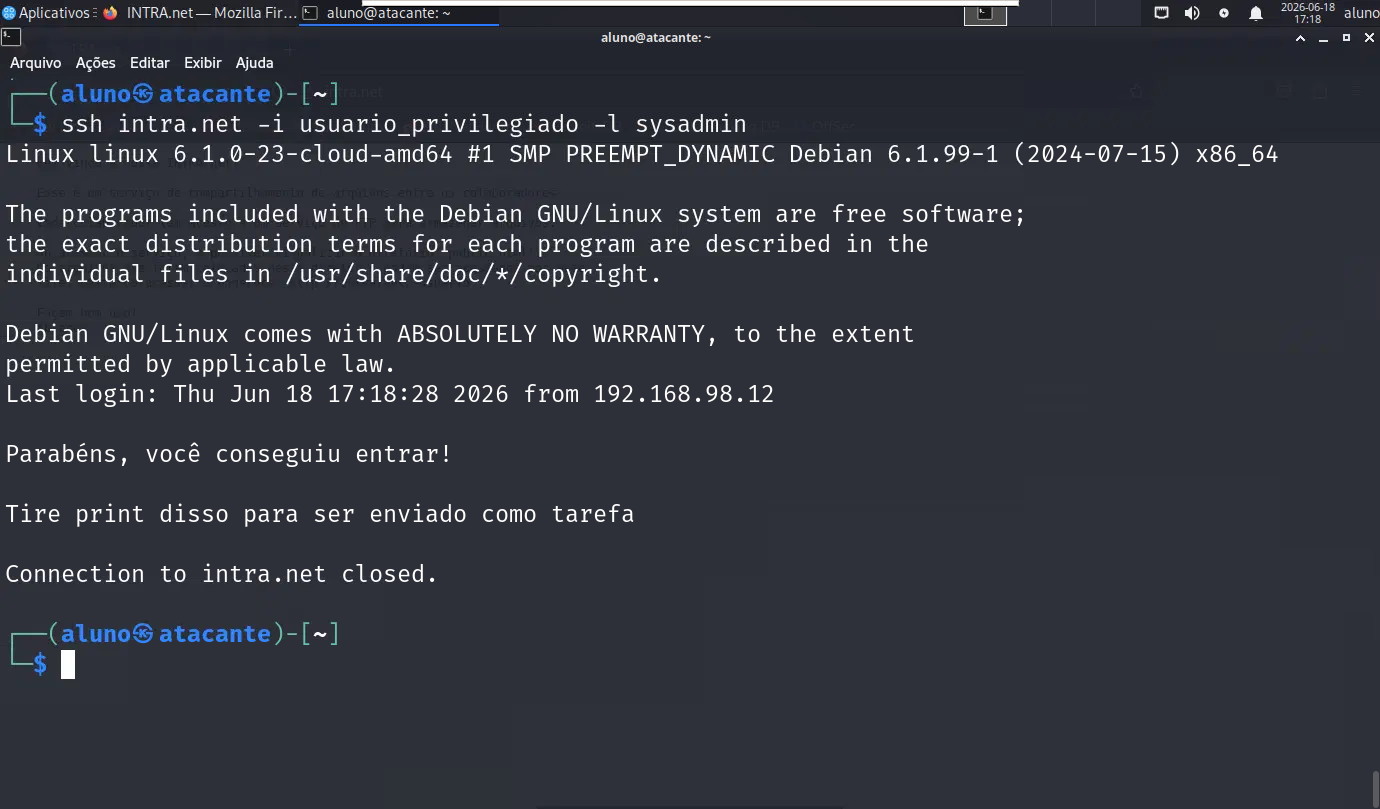
\includegraphics[width=0.95\textwidth]{./fig/login-ssh-privilegiado.png}
    \caption{Login realizado com sucesso utilizando a chave SSH encontrada e a
    conta privilegiada identificada durante a auditoria.}
\end{figure}

\subsection{Atividade 4 -- Geração de Wordlist por Expressão Regular}

\paragraph{}
Foi simulado um cenário de observação de padrões de senha utilizados por um
usuário da organização.

\paragraph{}
Com base nas características observadas, foi criada uma expressão regular
representando o padrão provável da senha.

\paragraph{}
A ferramenta \texttt{Exrex} foi utilizada para gerar uma wordlist contendo
apenas combinações compatíveis com o padrão identificado, reduzindo
significativamente o espaço de busca.

\paragraph{}
A wordlist gerada foi utilizada em um ataque automatizado contra um serviço de
autenticação HTTP, permitindo identificar as credenciais válidas do usuário
alvo.

\subsection{Atividade 5 -- Quebra de Hashes}

\paragraph{}
Foram utilizadas hashes obtidas anteriormente durante a exploração de uma
vulnerabilidade de SQL Injection.

\paragraph{}
Inicialmente foi realizada a identificação do algoritmo utilizado por meio das
ferramentas \texttt{hashid} e \texttt{Name-That-Hash}, concluindo que as hashes
utilizavam o algoritmo MD5.

\paragraph{}
Em seguida foi empregada a ferramenta \texttt{John the Ripper} para executar o
processo de quebra das hashes utilizando ataques baseados em wordlists.

\paragraph{}
O procedimento permitiu recuperar as senhas associadas às hashes fornecidas,
demonstrando os riscos da utilização de algoritmos de hash obsoletos para
armazenamento de credenciais.
